\section{Neural Network Types}
\label{sec:nnet_types}

\subsection{Feed Forward Neural Networks (Multilayer Perceptron)}

Feed forward neural layers is multidimensional generalization of perceptron. 
Generally, a neural layer might output multiple values (say $o \in \mathbb{R}^{1 \times d_o}$) as vector from input (say $x \in \mathbb{R}^{1 \times d_x}$). 
Such a setting forces parameter $W \in \mathbb{R}^{d_x \times d_o} $ to be a matrix. 
Moreover, activation function is not necessarily a step function. 
It can be any nonlinear function like sigmoid, tanh, ReLU etc. 
Feed Forward Neural Networks are the generalization of perceptron to approximate any function. 
Neural layers are stacked to construct deep feed forward neural network. 
It defines a nonlinear mapping $y=\phi(x;\theta)$ between input $x$ and output $y$, parametrized by $\theta$ that includes (learnable) parameters like weights, bias and possibly others if defined.

Assuming input signal is $x \in \mathbb{R}^{1 \times d_x}$ (output of previous layer), 
activation value of the layer ($h \in \mathbb{R}^{1 \times d_h}$) is calculated by linear transformation (weight $W$ and bias $b$) followed by nonlinear activation $\phi$, 
\begin{equation}
\label{eqn:mlpact}
h = \phi(x W + b),
\end{equation}
where $\phi$ is applied elementwise.

\subsection{Residual Feed Forward Neural Networks}

As Feed Forward Networks becomes deeper, optimizing weights gets difficult. 
Therefore, people come with the idea of residual connections~\cite{he_deep_2015}. 
For a fixed number of stacked layers (usually 2 which is single skip), input and output of the stack is summed up for next calculations. 
Replacing feed forward layers with other types yield different kind of residual network. 
The difference is demonstrated in \figref{fig:rffnn_ffnn}. 
Yellow blocks are layers where $\phi$ indicates layer has activation while empty ones are linear layers.

\begin{figure}
	\centering
	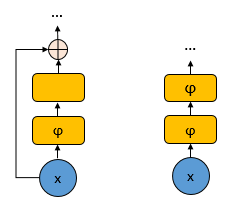
\includegraphics[width=0.5\textwidth]{figures/ml_theory/rffnn_vs_ffnn.png}
	\caption{Deep Feed Forward (left) and Deep Residual Feed Forward Network with single skip connection (right)}
	\label{fig:rffnn_ffnn}
\end{figure}

\subsection{Recurrent Neural Networks}

Recurrent Neural Networks (RNNs) \cite{rumelhart_learning_1986} are one type of neural network to process sequential data. 
It is specialized for data having sequential topology. 

In FFNN layer, output only depends on its input, while Recurrent Layer output depends on both input at time $t$ and its output in previous time step $t-1$. 

RNN can be thought as multiple copies of same network which passes message to its successor through time. 
A RNN layer is similar to a FFNN layer as in \eqref{eqn:mlpact}, 
except that input is concatenation of the output feedback and input itself.

Given an input sequence $x \in \mathbb{R}^{T \times d_x}$ with time length $T$, an output sequence $h \in \mathbb{R}^{T \times d_h}$ is evaluated recursively by 
\begin{equation}
\label{eqn:rnnact}
h_t = \phi(h_{t-1} \tilde{W} + x_t W + b),
\end{equation}
where nonlinear activation $\phi$ applied elementwise as in \eqref{eqn:mlpact} again. 
To begin with, the initial output $h_0$ can be either parametrized or assigned to a zero vector. A comparison between FFNN and RNN layer is visualized in \figref{fig:rnn_vs_ffnn}.

\begin{figure}
	\centering
	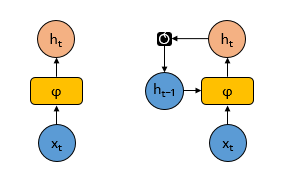
\includegraphics[width=0.5\textwidth]{figures/ml_theory/ffnn_vs_rnn.png}
	\caption{Feed Forward Layer (left) and Recurrent Layer (right) illustration~\cite{olah_understanding_2015}}
	\label{fig:rnn_vs_ffnn}
\end{figure}

\subsubsection{Long Short Term Memory}

Conventional RNNs have, in general, the problem with vanishing/exploding gradient \cite{olah_understanding_2015}. 
As the sequence gets longer, effect of initial inputs in sequence decreases. 
This causes a long term dependence problem. Furthermore, if information from initial inputs required, gradients either vanish or explode. 
In order to overcome this problem another architecture is developed: Long Short Term Memory (LSTM)~\cite{hochreiter_long_1997}. 

LSTM is a special type of RNN. 
It is explicitly designed to allow learning long-term dependencies. 
A single LSTM cell has four neural layers while a vanilla RNN layer has only one neural layer. 
In addition to the hidden state $h_t$, there is another state called cell state $C_t$. 
Information flow is controlled by three gates. 

\begin{figure}
	\centering
	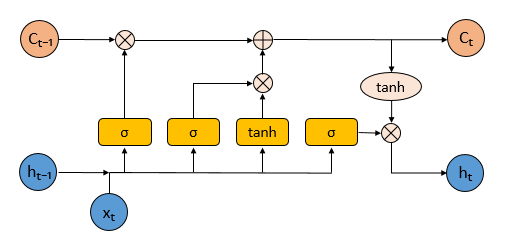
\includegraphics[width=0.98\textwidth]{figures/ml_theory/lstm_cell.png}
	\caption{LSTM Cell~\cite{olah_understanding_2015}}
	\label{fig:lstm_cell}
\end{figure}

\textbf{Forget Gate} controls past memory. 
According to input, past memory is either kept or forgotten. 
The sigmoid function ($\sigma$) is generally used as an activation function: 
\begin{equation}
\label{eqn:lstm_forget}
f_t = \sigma( [h_{t-1}; x_t] W_f + b_f).
\end{equation}

Hyperbolic tangent layer creates new candidate of cell state from the input:  
\begin{equation}
\label{eqn:lstm_cellstcand}
\hat{C}_t = \tanh( [h_{t-1}; x_t] W_C + b_C).
\end{equation}

\textbf{Input Gate} controls contribution from input to cell state (memory): 
\begin{equation}
\label{eqn:lstm_inp}
i_t = \sigma( [h_{t-1}; x_t] W_i + b_{i}).
\end{equation}
Once what are to be forgotten and added decided, cell state is updated accordingly, 
\begin{equation}
\label{eqn:lstm_cellstupt}
C_t = f_t \odot C_{t-1} + i_t \odot \hat{C}_t.
\end{equation}
using input gate and forget gate outputs. Note that $\odot$ is elementwise multiplication.

\textbf{Output Gate} controls which part of new cell state to be output: 
\begin{equation}
\label{eqn:lstm_out}
o_t = \sigma( [h_{t-1}; x_t] W_o + b_o).
\end{equation}

Finally, cell state is filtered by hyperbolic tangent to push values to be in $(-1,1)$ before evaluating the hidden state $h_t$ using output gate outputs: 
\begin{equation}
h_t = o_t \odot \tanh(C_t).
\end{equation}

\subsection{Attention Based Networks}

As stated earlier, recurrent neural networks are prone to forget long term dependencies. 
LSTM and other variants are invented to overcome such problems. 
However, they cannot attend specific parts of the input. 
Therefore, researchers come with the idea of weighted averaging all states through time where weights depends on both input and output. 
Let the input sequence $x \in \mathbb{R}^{T \times d_x}$ with time length $T$ be encoded to $h \in \mathbb{R}^{T \times d_h}$. 
The context vector is calculated using weight the vector $\alpha \in \mathbb{R}^{1 \times T}$ including a scalar for each time step, then attention output is, 
\begin{equation}
\mathrm{Attention}(q, h) = \alpha h. %\sum_{\tau=1}^{T} \alpha_{\tau} h_{\tau}.
\label{eq:attention_generic}
\end{equation}  

Attention weight $\alpha \in \mathbb{R}^{T}$ is calculated using hidden sequence
$h \in \mathbb{R}^{T \times d_H}$ and query $q \in \mathbb{R}^{1 \times d_Q}$ with a predefined a arbitrary function $\phi$ depending on choice. 
Query can be hidden state itself (self attention) or any input assumed to help attention weighting. 
In general form,  
\begin{equation}
\alpha = \phi(q, h; \theta_{\alpha}).
\end{equation}

\subsubsection{Transformer}

The Transformer was proposed in "Attention is All You Need"~ \cite{vaswani_attention_2017} paper. 
Unlike recurrent networks, this architecture is solely built on attention layers. 

A transformer layer consists of feed-forward and attention layers, which makes the mechanism special. 
Like RNNs, it can be used as both encoder and decoder. 
While encoder layers attend to itself, decoder layers attends both itself and encoded input. 

\textbf{Attention Layer} is a mapping from 3 vectors: query $Q \in \mathbb{R}^{T_q \times d_k}$, key $K \in \mathbb{R}^{T \times d_k}$ and value $V \in \mathbb{R}^{T \times d_v}$ to output, 
where $T$ is input time length, $T_q$ time length of query, $d_k$ and $d_v$ are embedding dimensions. 
Output is weighted sum of values $V$ through time dimension while weights are evaluated by compatibility metric of query $Q$ and key $K$. 
In vanilla transformer, compatibility of query and key is evaluated by dot product, normalizing by $\sqrt{d_k}$. 
For a query, dot product with all keys are evaluated, then softmax function is applied to get weights of values, 
\begin{equation}
\mathrm{Attention}(Q, K, V) = \mathrm{softmax}\bigg(\frac{Q K^{T}}{\sqrt{d_k}}\bigg) V.
\end{equation}
This approach is called Scaled Dot-product Attention. 

Instead of performing a single attention, \textbf{Multi-Head Attention} projects keys, queries and values linearly from $d_m$ dimensional vector space to $h$ different spaces using projection matrices. 
In this case, attention is performed $h$ times, and results are then concatenated and linearly projected to final values of the layer.
Projection matrices are model parameters, $W^Q_i \in \mathbb{R}^{d_m \times d_k}$, $W^K_i \in \mathbb{R}^{d_m \times d_k}$, $W^V_i \in \mathbb{R}^{d_m \times d_v}$ for $i=1,...,h$. 
Also output matrix is used to project multiple values into single one, $W^O \in \mathbb{R}^{h d_v \times d_m}$. Mathematically, 
\begin{equation}
\begin{split}
% It is better to write these as \DeclareMathOp
\mathrm{MHA}(Q,K,V) &=  \text{Concat}(\mathrm{head}_1, \mathrm{head}_2, ... \mathrm{head}_h)W^O \\
\mathrm{head}_i &=  \text{Attention}(QW^Q_i,KW^K_i,VW^V_i)
\end{split}.
\end{equation}
Scaled dot-product attention and Multi-Head attention are demonstrated in \figref{fig:att_and_mha}

\begin{figure}
	\centering
	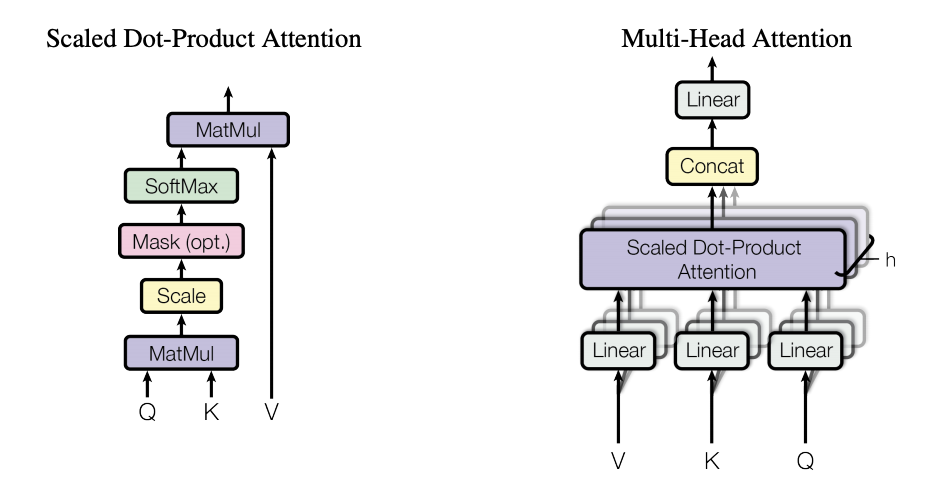
\includegraphics[width=0.98\textwidth]{figures/ml_theory/att.png}
	\caption{Scaled Dot-Product Attention (left) and Multi-Head Attention (right)~\cite{vaswani_attention_2017}}
	\label{fig:att_and_mha}
\end{figure}

A transformer layer contains \textbf{Feed Forward Layer}, containing two linear transformations ($W_1, b_1$ and $W_2, b_2$) with ReLU-like activation:
\begin{equation}
\mathrm{FFN}(x) = \text{ReLU}(x W_1 + b_1) W_2 + b_2.
\end{equation}

\textbf{Encoder Layer} starts with a residual self attention layer. 
Self attention means that query, key and value are the same vectors. 
This is followed by feed forward neural layer. 
Both sublayers are employed with resudial connection with layer normalization.
In other words, summation of layer input and output is passed through layer normalization: 
\begin{equation}
\begin{split}
a = & \mathrm{LN}(x + \mathrm{MHA}(x,x,x)), \\
y = & \mathrm{LN}(a + \mathrm{FFN}(a)).
\end{split}
\end{equation}

Apart from encoder layers; query, key and value inputs may vary depending on design. In general,
\begin{equation}
\begin{split}
a = & \mathrm{LN}(x + \mathrm{MHA}(q,k,v)), \\
y = & \mathrm{LN}(a + \mathrm{FFN}(a)).
\end{split}
\end{equation}

Since there are no recurrent or convolutional architecture in the model, sequential information needs to be embedded. 
For this purpose, \textbf{Positional encoding}s are used. 
They have same dimension with as the input $x$, so that input embeddings can be added to at the beginning of encoder or decoder stacks. 
Let the positional encoding $\mathrm{PE} \in \mathbb{R}^{T \times d_m}$.
For $t$th position in time, and $i$th position in embedding axis ($i \in \mathbb{N}$), $\mathrm{PE}$ is defined as follows: 
\begin{equation}
\mathrm{PE}_{t,i} = 
\begin{cases}
\sin(t/10000^{i/d_m}),   & \text{if } i \equiv 0 \pmod 2 ,\\
\cos(t/10000^{(i-1)/d_m}),   & \text{if } i \equiv 1 \pmod 2 ,
\end{cases}
\end{equation}
as proposed in the original paper \cite{vaswani_attention_2017}. 

\subsubsection{Pre-Layer Normalized Transformer}

Original transformer architecture includes layer normalization operations after attention and feed-forward layers. 
It is unstable since the values of gradients of output layers are high. 
Pre-Layer Normalized Transformer is proposed by \cite{xiong_layer_2020} by carrying layer normalization operation to in front of attention and feed-forward layers. 
Moreover, Parisotto et al. Xiong et al.~ \cite{parisotto_stabilizing_2019} propose gated transformer which also includes layer normalizations before attention and feedforward layer. 
They also state that although gated architecture improves many reinforcement learning (RL) tasks drastically, and non-gated pre-layer normalized transformer are also much better than vanilla transformer. 

In pre-layer normalized transformer, encoder equations are: 
\begin{equation}
\begin{split}
a = & x+ \mathrm{MHA}(\mathrm{LN}(x),\mathrm{LN}(x),\mathrm{LN}(x)) \\
y = & a + \mathrm{FFN}(\mathrm{LN}(a))
\end{split}.
\end{equation}

A simple pre-layer normalized transformer encoder layer is demonstrated in \figref{fig:pre_trsf}. 
The difference between post-layer and pre-layer transformer encoders are also visualized in \figref{fig:post_pre_trsf}

\begin{figure}
	\centering
	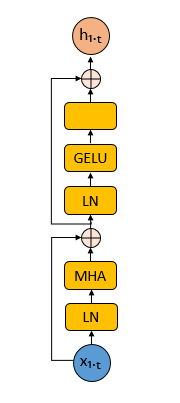
\includegraphics[width=0.3\textwidth]{figures/ml_theory/transformer_block.png}
	\caption{Pre-LN Transformer encoder layer with GELU activation}
	\label{fig:pre_trsf}
\end{figure}

\begin{figure}
	\centering
	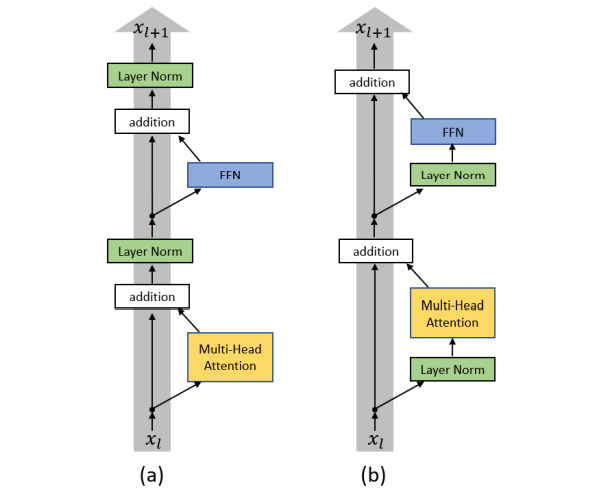
\includegraphics[width=0.7\textwidth]{figures/ml_theory/post_pre_trsf.png}
	\caption{(a) Post-LN Transformer layer, (b) Pre-LN Transformer
		layer~\cite{xiong_layer_2020}}
	\label{fig:post_pre_trsf}
\end{figure}
